\documentclass[11pt,letterpaper]{article}
\usepackage[margin=.75in]{geometry}
\usepackage{amsmath}
\usepackage{graphicx}
\usepackage{amssymb} \usepackage{natbib}
\usepackage{float} \usepackage{appendix}
\usepackage{hyperref}
\usepackage{mathrsfs}
\floatstyle{ruled} \restylefloat{table} \restylefloat{figure}
\bibliographystyle{unsrtnat}

\newcommand{\floatintro}[1]{
  
  \vspace*{0.1in}
  
  {\footnotesize

    #1
    
  }
  
  \vspace*{0.1in} }
\newcommand{\Hline}{\noindent\rule{17cm}{0.5pt}} \title{Homework 6:
  Industrial Organisation} \author{Dhananjay Ghei} \date{December 11,
  2018}
\begin{document}
\maketitle
\textit{N.B. The code for this exercise was written in
\texttt{R} and is available on my Github
account. \url{www.github.com/dhananjayghei/io_estimation}.}

\section*{Some basics}
\begin{enumerate}
\item Read the data into a statistical package and look at summary
statistics to convince yourself that the data was read in
correctly. Try a simple OLS regression of log(QUANTITY) on a constant,
log(PRICE), LAKES, and (twelve of) the seasonal dummy variables. If
you were to view this as an estimate of a demand curve what would the
price elasticity of demand be? Why does this number seem unreasonable?
\\ \Hline \\
Table \ref{tab:sumstats} shows the summary statistics from Porter's
data set. The number are the same as in Table II of Porter. Thus, the
data has been read in correctly. 
\begin{table}[htbp!]
  \floatintro{The table shows the summary statistics from Porter's
    data set.}
  \centering
  \input{./tables/sumstats_porter_float.gen}
  \caption{Summary statistics}
  \label{tab:sumstats}
\end{table}
Figure \ref{fig:fig1} shows the plot of price as a function of time
(in weeks). This replicates the Figure I from Porter. 
\begin{figure}[htbp!]
  \floatintro{The figure shows the plot of price as a function of
    time. The time is in weeks starting from Jan 1, 1980. } \centering
  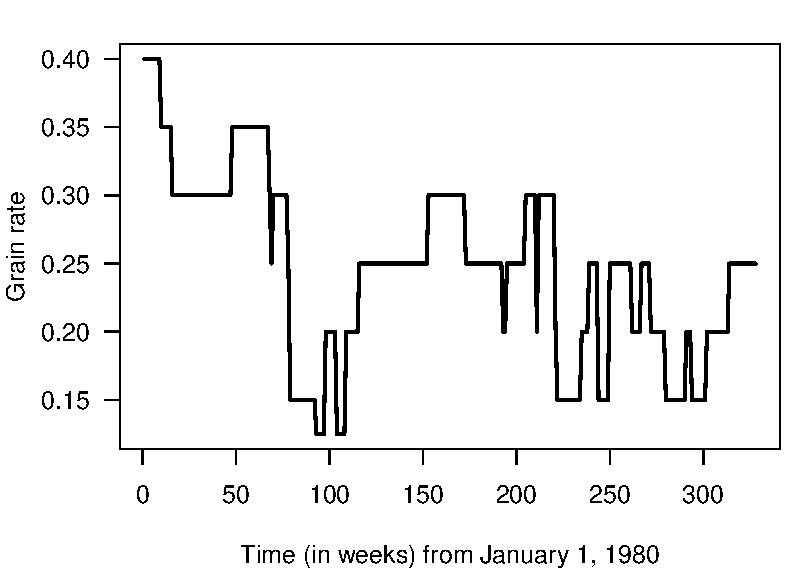
\includegraphics[scale=.6]{./pics/fig1_porter.pdf}
  \caption{Plot of price as a function of time}
  \label{fig:fig1}
\end{figure}

Column I of Table \ref{tab:demand} shows the OLS estimates of the
demand equation. Demand elasticity from OLS is equal to 0.639. The
demand is inelastic. This seems unreasonable because if we expect JEC
to act as a monopolist, prices should go to infinity. One potential
reason for this is that the price is endogenous which gives the
estimate of elasticity to be biased towards zero.
\item Try doing the regression instead using instrumental variable
  with the COLLUSION variable as the instrument for PRICE. How does
  the reported price elasticity change. Is the estimate closer to that
  in Porter's paper or that in Ellison's paper and why? How do you
  interpret the coefficient on the LAKES variable? On the seasonal
  dummies? What is the R-squared of the regression and what do you
  make of it? \\ \Hline \\
  Column II of Table \ref{tab:demand} shows the IV estimate using
  collusion as the instrument for price. Instrumenting increases the
  estimated demand elasticity from .639 to .867. This is closer to the
  Ellison's paper. For the Lakes variable, going from 0 to 1 indicates
  the opening of great lakes for navigation. The difference in
  expected log quantities is given by $\log(Q_1) - \log(Q_0) = -.423$
  which gives $\frac{Q_1}{Q_0} = \exp(-.423) = .66$. Thus, opening of
  lakes lead to a reduction of 34\% in the quantity shipped given
  price.  The interpretation on the seasonal dummies is similar to the
  one for lakes. In fact, there are some seasonal dummies which show
  statistical significance.  In the IV case, the R-square coefficients
  do not hold much significance. This is the reason we do not get an
  F-stat for the two regressions.

\item Try the regression with the DM1-DM4 and COLLUSION as instruments
  for price. Do the estimates ``improve'' in any way? \\ \Hline \\
  Column III of Table \ref{tab:demand} shows the instrumental variable
  estimation using the collusion variable and the dummy variable as
  instrument. This does not help in changing the elasticity.
  \begin{table}
    \floatintro{The table shows the demand estimation using OLS and
      instrumental variable estimation. Column I shows the results of
      OLS, Column II shows the results of IV using collusion as an
      instrument for price and Column III shows the results of IV
      using collusion and the dummies (DM1-DM4) as instruments for
      price.}
    \centering
    \resizebox{.6\textwidth}{!}{
      \input{./tables/porter_demand.gen}}
    \caption{Demand estimation}
    \label{tab:demand}
  \end{table}
\item Estimate a supply equation as in Porter and Ellison using the
  LAKES variable as an instrument for quantity. What does the
  magnitude of the coefficient on COLLUSION tell us about the effect
  of collusion on prices? What might the coefficient on QUANTITY in
  this regression indicate about the nature of costs in the JEC? \\
  \Hline \\
  Table \ref{tab:supply} shows the estimation of supply equation using
  OLS and IV where the lakes variables is used as an instrument for
  quantity.  The coefficient on collusion in the case of IV is
  0.368. Thus, the ratio of prices is equal to $\exp(.368) = 1.44$ and
  therefore, the prices are 44\% higher in collusion. If you compare
  the results from Column II of Table \ref{tab:supply} with Column II
  of Table III from Porter, they are pretty similar even though we do
  not have the estimated dummy variable as in Porter. The coefficient
  on quantity is $0.253$ which is positive but not statistically
  significant.
  \begin{table}
    \floatintro{The table shows the supply side estimation using OLS and
      instrumental variable estimation. Column I shows the results of OLS,
      Column II shows the results of IV using the lakes variable as an
      instrument for quantity.}
    \centering
    \resizebox{.35\textwidth}{!}{
      \input{./tables/porter_supply.gen}}
    \caption{Supply estimation}
    \label{tab:supply}
  \end{table}
\end{enumerate}

\section*{Model derivation and interpretation}
\begin{enumerate}
\item Suppose that rather than the log-log specification of demand
  you've been using so far, you tried others and found that a linear
  specification of demand like
  \begin{align*}
    Q_t = \alpha_0 + \alpha_1 P_t + \alpha_2 Lakes_t + u_t
  \end{align*}
  seemed most appropriate. Show that for this demand curve the optimal
  price for a monopolist with a constant marginal cost of $c$ to set
  is
  \begin{align*}
    P_t = c - \frac{1}{\alpha_1} Q_t
  \end{align*}
  Given this result, what functional form would you choose for the
  supply curve in this model? \\ \Hline \\
  The monopolist will solve:
  \begin{align*}
    \max_p (p-c)Q
  \end{align*}
  The first order condition is given by:
  $(p-c) \frac{\partial Q}{\partial p} + Q = 0$. From the demand
  function, we know that $\frac{\partial Q}{\partial p} = \alpha_1$,
  so we have $p = c - \frac{1}{\alpha}Q$.
\item What pricing rule would result with this demand curve if the
  industry instead consisted of perfectly competitive firms with total
  costs of the form $c(Q_t) = c_0Q_t + c_1Q_t^2$ setting price equal
  to marginal cost? Could one use an approach like Porter's to
  distinguish between these two models of behavior? Talk about why
  this is an important question. \\ \Hline \\
  If the industry was perfectly competitive, then the firms would
  price at marginal cost. Therefore, the supply equation will be:
  $p_t = c_0 + 2c_1Q_t$.
\end{enumerate}
\section*{Causes of price wars}
\begin{enumerate}
\item Using the collusion variable generate an indicator variable for
  the start of a price war. Perform a probit regression with this
  indicator as a dependent variable and with QUANTITY, LAKES, and
  DM1-DM4 (or a subset thereof) as explanatory variables. What
  inferences might you want to draw about whether price wars are more
  likely to occur in booms from the coefficients on the first two
  variables? Why are these variables not really the right ones to be
  using in the equation? \\ \Hline \\
  I construct the indicator variable for price war directly from the
  collusion variable. Price wars is equal to one when Collusion shifts
  from 1 to 0 and 0 otherwise. This gives us 11 events of price
  wars. As a result, we have very little variation in our dependent
  variable.\\
  Table \ref{tab:probit} shows the estimation from probit
  results. Heteroskedasticity consistent standard errors are used
  given the relatively smaller sample. The dummies turn out to be
  significant, whereas the lakes and quantity variable do not turn out
  to be significant.
  \begin{table}[htbp!]
    \floatintro{The table shows the results from probit
      estimation. Heteroskeadsticity consistent standard errors are used
      in the analysis.}
    \centering
    \resizebox{.45\textwidth}{!}{
      \input{./tables/probit_porter.gen}}
  \caption{Cause of price wars}
  \label{tab:probit}
\end{table}
\end{enumerate}
% \newpage
% \bibliography{IOpapers}

\end{document}
